\begin{pages}
    \begin{Rightside}
    \selectlanguage{greek}
        \beginnumbering
        \pstart[
        			\chapter{Ἡ Ἱερουσαλὴμ ἡ νέα}
        			\markboth{The New Jerusalem}
				]		
		\renewcommand{\LettrineFontHook}{\PHtitl}
		\lettrine[lines=3]{Κ}{αὶ} εἶδον οὐρανὸν καινὸν καὶ γῆν καινήν· ὁ γὰρ πρῶτος οὐρανὸς καὶ ἡ πρώτη γῆ ἀπῆλθαν, καὶ ἡ θάλασσα οὐκ ἔστιν ἔτι. καὶ τὴν πόλιν τὴν ἁγίαν Ἱερουσαλὴμ καινὴν εἶδον καταβαίνουσαν ἐκ τοῦ οὐρανοῦ ἀπὸ τοῦ Θεοῦ, ἡτοιμασμένην ὡς νύμφην κεκοσμημένην τῷ ἀνδρὶ αὐτῆς. καὶ ἤκουσα φωνῆς μεγάλης ἐκ τοῦ θρόνου λεγούσης Ἰδοὺ ἡ σκηνὴ τοῦ Θεοῦ μετὰ τῶν ἀνθρώπων, καὶ σκηνώσει μετ’ αὐτῶν, καὶ αὐτοὶ λαοὶ αὐτοῦ ἔσονται, καὶ αὐτὸς ὁ Θεὸς μετ’ αὐτῶν ἔσται, καὶ ἐξαλείψει πᾶν δάκρυον ἐκ τῶν ὀφθαλμῶν αὐτῶν, καὶ ὁ θάνατος οὐκ ἔσται ἔτι, οὔτε πένθος οὔτε κραυγὴ οὔτε πόνος οὐκ ἔσται ἔτι· ὅτι τὰ πρῶτα ἀπῆλθαν. 
		\pend
		\pstart
		καὶ εἶπεν ὁ καθήμενος ἐπὶ τῷ θρόνῳ Ἰδοὺ καινὰ ποιῶ πάντα. καὶ λέγει Γράψον, ὅτι οὗτοι οἱ λόγοι πιστοὶ καὶ ἀληθινοί εἰσιν. καὶ εἶπέν μοι Γέγοναν. ἐγὼ τὸ Ἄλφα καὶ τὸ Ὦ, ἡ ἀρχὴ καὶ τὸ τέλος. ἐγὼ τῷ διψῶντι δώσω ἐκ τῆς πηγῆς τοῦ ὕδατος τῆς ζωῆς δωρεάν. ὁ νικῶν κληρονομήσει ταῦτα, καὶ ἔσομαι αὐτῷ Θεὸς καὶ αὐτὸς ἔσται μοι υἱός. τοῖς δὲ δειλοῖς καὶ ἀπίστοις καὶ ἐβδελυγμένοις καὶ φονεῦσιν καὶ πόρνοις καὶ φαρμάκοις καὶ εἰδωλολάτραις καὶ πᾶσιν τοῖς ψευδέσιν τὸ μέρος αὐτῶν ἐν τῇ λίμνῃ τῇ καιομένῃ πυρὶ καὶ θείῳ, ὅ ἐστιν ὁ θάνατος ὁ δεύτερος.
		\pend
		\pstart
		Καὶ ἦλθεν εἷς ἐκ τῶν ἑπτὰ ἀγγέλων τῶν ἐχόντων τὰς ἑπτὰ φιάλας, τῶν γεμόντων τῶν ἑπτὰ πληγῶν τῶν ἐσχάτων, καὶ ἐλάλησεν μετ’ ἐμοῦ λέγων Δεῦρο, δείξω σοι τὴν νύμφην τὴν γυναῖκα τοῦ ἀρνίου. καὶ ἀπήνεγκέν με ἐν Πνεύματι ἐπὶ ὄρος μέγα καὶ ὑψηλόν, καὶ ἔδειξέν μοι τὴν πόλιν τὴν ἁγίαν Ἱερουσαλὴμ καταβαίνουσαν ἐκ τοῦ οὐρανοῦ ἀπὸ τοῦ Θεοῦ, ἔχουσαν τὴν δόξαν τοῦ Θεοῦ· ὁ φωστὴρ αὐτῆς ὅμοιος λίθῳ τιμιωτάτῳ, ὡς λίθῳ ἰάσπιδι κρυσταλλίζοντι· 
		\pend
		\pstart
		ἔχουσα τεῖχος μέγα καὶ ὑψηλόν, ἔχουσα πυλῶνας δώδεκα, καὶ ἐπὶ τοῖς πυλῶσιν ἀγγέλους δώδεκα, καὶ ὀνόματα ἐπιγεγραμμένα, ἅ ἐστιν τῶν δώδεκα φυλῶν υἱῶν Ἰσραήλ. ἀπὸ ἀνατολῆς πυλῶνες τρεῖς, καὶ ἀπὸ βορρᾶ πυλῶνες τρεῖς, καὶ ἀπὸ νότου πυλῶνες τρεῖς, καὶ ἀπὸ δυσμῶν πυλῶνες τρεῖς. καὶ τὸ τεῖχος τῆς πόλεως ἔχων θεμελίους δώδεκα, καὶ ἐπ’ αὐτῶν δώδεκα ὀνόματα τῶν δώδεκα ἀποστόλων τοῦ Ἀρνίου. 
		\pend
		\pstart
		Καὶ ὁ λαλῶν μετ’ ἐμοῦ εἶχεν μέτρον κάλαμον χρυσοῦν, ἵνα μετρήσῃ τὴν πόλιν καὶ τοὺς πυλῶνας αὐτῆς καὶ τὸ τεῖχος αὐτῆς. καὶ ἡ πόλις τετράγωνος κεῖται, καὶ τὸ μῆκος αὐτῆς ὅσον τὸ πλάτος. καὶ ἐμέτρησεν τὴν πόλιν τῷ καλάμῳ ἐπὶ σταδίων δώδεκα χιλιάδων· τὸ μῆκος καὶ τὸ πλάτος καὶ τὸ ὕψος αὐτῆς ἴσα ἐστίν. καὶ ἐμέτρησεν τὸ τεῖχος αὐτῆς ἑκατὸν τεσσεράκοντα τεσσάρων πηχῶν, μέτρον ἀνθρώπου, ὅ ἐστιν ἀγγέλου. καὶ ἡ ἐνδώμησις τοῦ τείχους αὐτῆς ἴασπις, καὶ ἡ πόλις χρυσίον καθαρὸν ὅμοιον ὑάλῳ καθαρῷ. 
		\pend
		\pstart
		οἱ θεμέλιοι τοῦ τείχους τῆς πόλεως παντὶ λίθῳ τιμίῳ κεκοσμημένοι· ὁ θεμέλιος ὁ πρῶτος ἴασπις, ὁ δεύτερος σάπφειρος, ὁ τρίτος χαλκηδών, ὁ τέταρτος σμάραγδος, ὁ πέμπτος σαρδόνυξ, ὁ ἕκτος σάρδιον, ὁ ἕβδομος χρυσόλιθος, ὁ ὄγδοος βήρυλλος, ὁ ἔνατος τοπάζιον, ὁ δέκατος χρυσόπρασος, ὁ ἑνδέκατος ὑάκινθος, ὁ δωδέκατος ἀμέθυστος. καὶ οἱ δώδεκα πυλῶνες δώδεκα μαργαρῖται· ἀνὰ εἷς ἕκαστος τῶν πυλώνων ἦν ἐξ ἑνὸς μαργαρίτου. καὶ ἡ πλατεῖα τῆς πόλεως χρυσίον καθαρὸν ὡς ὕαλος διαυγής. 
		\pend
		\pstart
		Καὶ ναὸν οὐκ εἶδον ἐν αὐτῇ· ὁ γὰρ Κύριος ὁ Θεὸς ὁ Παντοκράτωρ ναὸς αὐτῆς ἐστιν, καὶ τὸ Ἀρνίον. καὶ ἡ πόλις οὐ χρείαν ἔχει τοῦ ἡλίου οὐδὲ τῆς σελήνης, ἵνα φαίνωσιν αὐτῇ· ἡ γὰρ δόξα τοῦ Θεοῦ ἐφώτισεν αὐτήν, καὶ ὁ λύχνος αὐτῆς τὸ Ἀρνίον. καὶ περιπατήσουσιν τὰ ἔθνη διὰ τοῦ φωτὸς αὐτῆς, καὶ οἱ βασιλεῖς τῆς γῆς φέρουσιν τὴν δόξαν αὐτῶν εἰς αὐτήν· καὶ οἱ πυλῶνες αὐτῆς οὐ μὴ κλεισθῶσιν ἡμέρας, νὺξ γὰρ οὐκ ἔσται ἐκεῖ· καὶ οἴσουσιν τὴν δόξαν καὶ τὴν τιμὴν τῶν ἐθνῶν εἰς αὐτήν. καὶ οὐ μὴ εἰσέλθῃ εἰς αὐτὴν πᾶν κοινὸν καὶ ὁ ποιῶν βδέλυγμα καὶ ψεῦδος, εἰ μὴ οἱ γεγραμμένοι ἐν τῷ βιβλίῳ τῆς ζωῆς τοῦ Ἀρνίου.	
		\pend
        \endnumbering
    \end{Rightside}
    \begin{Leftside}
        \beginnumbering
        \pstart[
        			\chapter{The New Jerusalem}
				]		
		\renewcommand{\LettrineFontHook}{\Zallmanfamily}
		\lettrine[lines=3]{A}{nd} I saw a new Heaven and a new Earth; for the first Heaven and the first Earth have departed (left) and the sea is no more. And the new holy city (of) Jerusalem I saw descending out of Heaven from God (and it was) prepared as a bride (is) for her husband (man). And I heard a great voice from the throne saying, “Behold! The tabernacle (tent) of God (is?) with the humans and He will live with them and they will be His people; and God himself will be with them. And He will wipe away every tear from their eyes and there will no longer be either death nor mourning nor weeping nor pains (toils, hardship) — for the first things have departed (gone away, left). 
		\pend
		\pstart
		And He who sits upon the throne said, “Behold! I make everything new (all things new).” And He says, “Write that (because?) these words are faithful and true.” And He said to me, “They (i. e. these things) have (now) happened (it is done). I am the Alpha and the Omega, the beginning and the end. I shall give the thirsty from the spring (fountain) of water of life freely. The victor shall inherit (all) this and I will be God to him and he will be a son to Me. But to the fearful (cowardly) and unbelieving and detestable (abominable) and murderers and those who are sexually immoral; and (to) the sorcerers and those worshipping idols and to every liar: their part is in the lake burning with fire and brimstone (sulphur), which is the second death.”
		\pend
		\pstart
		And there came (forth) one of the seven angels — the ones having the seven vials filled with the last seven plagues —and he spoke to me saying, “Come. I will show you the wife — the woman — of the Lamb.” And he carried me away in Spirit onto a great and high mountain; and he showed me the holy city Jerusalem — (the one) having the glory of God — descending out of Heaven from God. (And) its splendour was akin to (that of) a precious stone, (or) like (that of) crystal clear piece of jasper. 
		\pend
		\pstart
		And it had a great and tall wall, and it had twelve gates and upon the gates (there were) twelve angels and names (were) inscribed (upon them), (namely the names) which are (those) of the twelve tribes of Israel — three gates in the West(ern) part, three gates in the North(ern) part, three gates in the South(ern) part and three gates in the West(ern) part. And the city’s wall had twelve foundations and (written) upon them were the twelve names of the apostles of the Lamb. 
		\pend
		\pstart
		And (whilst he was) speaking to me, he had (in his hands) a golden measuring rod so that he may measure the city and its gates and its wall. And the city is laid (out as a) square and its length is as great as its breadth. And he measured the city with the rod at twelve-thousand stadia (roughly 2,100 km); its length and its breadth and its height are equal (in length). And he measured its wall at one-hundred forty-four cubits (roughly 72 m), the measure of a man, which is of the angel. And the material (out) of (which) the wall (was built) was jasper and the city was (made out of) pure gold, as a fine crystal. 
		\pend
		\pstart
		And the foundations of the wall were adorned with all (kinds of) precious stones: the first foundation is (made out of) jasper, the second is (made out of) sapphire, the third is (made out of) chalcedony, the fourth is (made out of) emerald, the fifth is (made out of) sardonyx, the sixth is (made out of) carnelian, the seventh is (made out of) chrysolite, the eight is (made out of) beryl, the ninth is (made out of) topaz, the tenth is (made out of) chrysoprase, the eleventh is (made out of) jacinth, and the twelfth is (made out of) amethyst. And the twelve gates are twelve pearls (and) each of the gates was (made out) of one (of the) pearls. And the street of the city (is made of) pure gold, like a transparent crystal.
		\pend
		\pstart
		And I did not see any people in it, for the Lord God — the Almighty — is its people, and (so is) the Lamb. And the city has no need for the Sun, nor for the Moon, so that they may shine in it. For the glory of God illuminated it, and its lamp is the Lamb. And the nations will walk (through the city) through its (because of its) light, and the kings of the Earth carry their glory into it. And its gates may not be shut during the day, for there shall not be any night there. And they shall bring the glory and honour of the nations into it. And no unclean person nor any liar or person who does detestable things may enter it, except for the ones who are written in the Lamb’s book of life. 
		\pend
        \endnumbering
    \end{Leftside}

\end{pages} 
\Pages

\clearpage
\thispagestyle{empty}
\null\vfill
\settowidth\longest{\huge\itshape […] and when I turned around I saw}
\begin{center}
\parbox{\longest}{%
  \raggedright{\huge\itshape%
    ``Quote here.'' \par\bigskip
  }
  \raggedleft\Large\MakeUppercase{``The Celestial City and the River of Bliss'' — John Martin, 1841}\par%
}
\vfill\vfill
\clearpage\newpage
\end{center}
\newpage
\thispagestyle{empty}
\begin{center}
	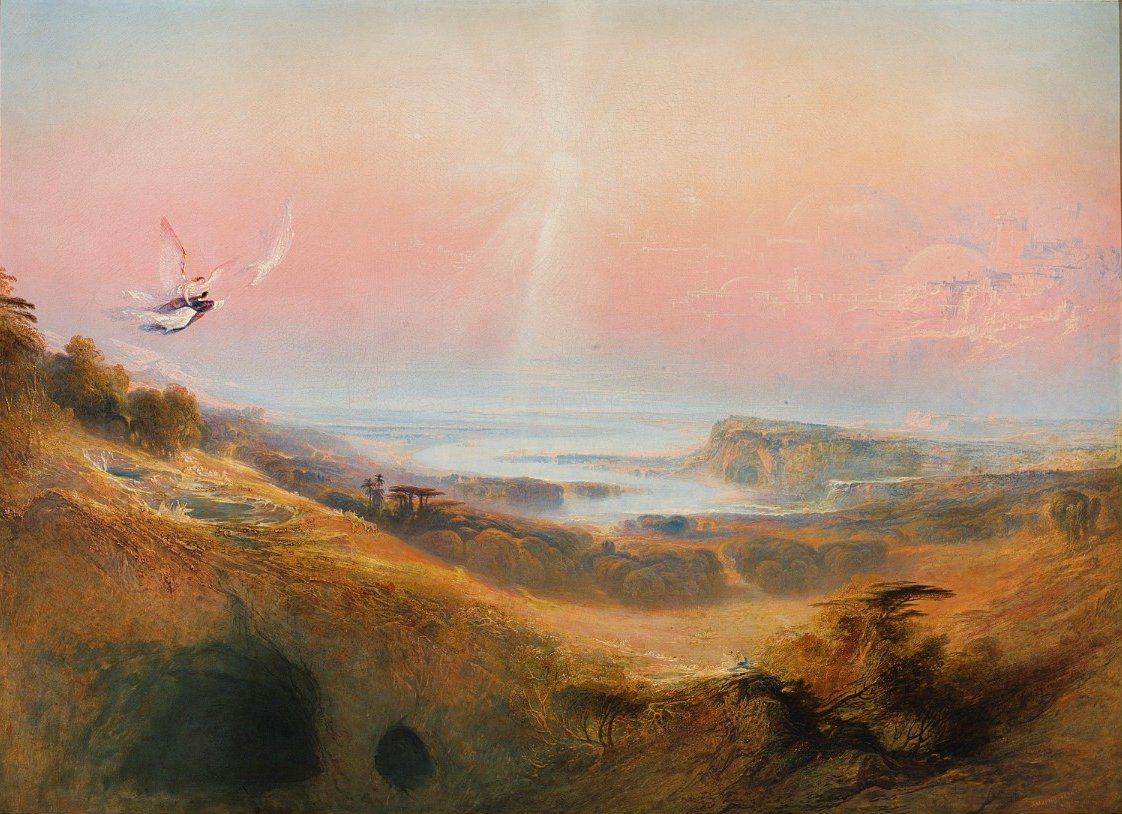
\includegraphics[angle=90, width=1\textwidth]{images/illustrations/johnmartinnewjerusalem}
\end{center}